\chapter{The State of Patient Simulators}
\label{ch:simulators-sota}

\section{Introduction}
\label{sec:intro}

Patient simulators have been applied extensively in nursing education \cite{didactic-sims1,didactic-sims2,didactic-sims3}, both as physical mannequins and as digital patient simulation software \cite{didactic-virtual}.
However, patient simulators have another important application: they can be used to predict how patients' health would respond to various treatments and thus evaluate proposals for novel treatment strategies.
And now, with the advent of machine learning, one can use reinforcement learning \cite{healthcare-rl}, genetic programming or both (see chapter \ref{ch:neurogen}) to generate treatment strategies that lead to the best outcomes for the patient according to a certain simulator.
In this chapter we review the field of interactive patient simulators and evaluate their potential to be used for automated treatment discovery.

\subsection{Scope of this survey}
\label{sec:scope}

This survey only includes interactive patient simulators where a (human or software) agent communicates its clinical intervention decisions to the simulator and the simulator, in turn,
\begin{enumerate}
    \item \emph{Predicts} future patient state given current patient state and clinical interventions.
    \item \emph{Rewards} or punishes (negatively rewards) that judges if the result of the treatment is positive or negative. The model can be as simple as just negatively rewarding patient deaths or as complex as using the predictions of the \emph{prediction model} to help the agent recognize during the episode whether they are on the right track to a positive outcome.
\end{enumerate}

Any interactive simulator with a prediction model and a reward model (and thus, all simulators in this chapter) can be represented as {\em Episodic Partially Observable Markov Decision Process} (EPOMDP) as described in chapter \ref{ch:neurogen}:

\begin{multline}
M = (\mathcal{S}_{nt}, \mathcal{S}_t, \mathcal{A}, \mathcal{O}, p_o(o | s, a), p_s(s_\text{next} | s_\text{prev}, a), p_r(r | s, a), p_\text{init}(s))
\end{multline}

Here, $\mathcal{S}_{nt}$ is the set of {\em non-terminal patient states}. $\mathcal{S}_{t}$ is the set of {\em terminal patient states} (death, discharge from hospital or end of outpatient treatment) such that getting to one of these states signifies the end of an episode. 
$\mathcal{A}$ is the set of {\em actions} that the learning agent can perform, and $\mathcal{O}$ is the set of {\em observations} about the current state that the agent can make. 
Distributions $p_o$, $p_s$ and $p_\text{init}$ represent the simulator's prediction model, while $p_r$ represents the reward model.

Markov Decision Processes are a standard formalism in the field of Reinforcement Learning \cite{suttonReinforcementLearningSecond2018}, so standard RL algorithms can be used in conjunction with any simulator from this chapter for treatment discovery.

There are 2 notable examples of systems that can be referred to as patient simulators, but do not make it easy to evaluate treatment strategies and fall outside the scope of this survey: 
\begin{enumerate}
    \item prediction models without a reward model
    \item synthetic data generators \cite{datagens}
\end{enumerate}

They former are tools like HumMod \cite{hummod} that help predict how change in one variable of patient health can affect another, for instance, how digoxin intake affects blood pressure.
A reward model is absolutely necessary for the application area that we focus on in this chapter - development and validation of treatment strategies.
Developing it is also a non-trivial problem in its own right - which health outcomes are considered \emph{good} depends on severity of the patient's condition (\emph{alive} is a sufficiently successful outcome for the most severe conditions, but not for others) as well as the patient's own preferences \cite{patpreferences1,patpreferences2}.
Thus, we view prediction models as components that can be used to develop a full simulator in the future.

The latter simulate clinical scenarios by generating samples of clinical histories.
They provide a privacy-preserving way to generate a lot of training data for treatment discovery \cite{privacy1,privacy2,privacy3,privacy4}, however, they do not model counterfactuals. That is, they do not answer questions of the sort "How would the patient's health respond to decision X"? For example, Synthea \cite{synthea} is a framework for generation of entire synthetic Electronic Health Records, EHRs, of patients, from the first to the last patient encounter, but the system does not provide ways to test alternative interventions on patients. 

\subsection{Simulators as models}

What makes an \emph{effective} patient simulator? 
We argue that there are two use cases for a patient simulator: {\sl modeling} and {\sl benchmarking}, with divergent effectiveness criteria.

\begin{figure}
    \centering
    
\includegraphics[width=\linewidth]{sim.png}
    \caption{Trust graph of simulator as a model}
    \label{fig:model}
\end{figure}

Firstly, a simulator can be used as a \emph{patient model} aiming to represent the real world evolution of patient health in response to various treatments as closely as possible.
The effectiveness criterion for a patient model is simple - \emph{accuracy}.
Accuracy can be measured by comparing the simulator's predictions against a dataset of clinical histories.
One metric in particular that has been used for simulator validation is \emph{mean predictive error over dynamic transitions} \cite{mdpe}.
If the simulator was obtained with machine learning, the data also has to be different from the training data: a different dataset or a holdout set can be used for that purpose.

The trust graph (see figure \ref{fig:model}) for a model is equally simple: if the data used for development of the simulator is a representative sample of the true distribution of the patients and the methodology used to turn build an interactive simulator based on these data is sound, the simulator is an accurate representation of a real world patient.
And if the training algorithm used to discover the optimal treatment under this simulator is sound, the resulting treatment strategy can be trusted as well.
Unfortunately, these conditions often hold only partially, or do not hold at all.

\subsection{Common biases}
\label{sec:bias}

One type of bias, present in most data-driven healthcare simulators is \emph{sampling bias}.
If patient data is used to develop a simulator, this data is a sample (and, potentially, a biased sample) of the patient population that may or may not represent the population accurately.
This problem is exacerbated by a profound shortage of healthcare datasets available to the research community.
The biggest currently available dataset is MIMIC-IV \cite{mimic} - a large database of electronic health records in intensive care.
However, MIMIC-IV was collected in one hospital in Boston and thus represents a demographically biased sample of the population.
This bias is likely to percolate into any simulator developed based on MIMIC-IV.

But the most crippling type of simulator bias that makes many simulators completely unsuitable to serve as patient models is \emph{confirmation bias}.
\emph{Confirmation bias} occurs when the developers of a simulator are aware of state of the art clinical practices and, intentionally or unintentionally, develop a simulator that rewards them and punishes alternatives.  
In \emph{didactic} simulators used for education of clinical professionals, confirmation bias exists by design: students are, after all, trained to follow established clinical protocols.
For a particular example of intentional confirmation bias in simulator design see \emph{Virtu-ALS} (section \ref{sec:virtu-als}). 
In this simulator, a decision that violates the existing emergence care protocol will be registered as a mistake, explained as such to the student, and \emph{not actually implemented}.

\subsection{Simulators as benchmarks}

\begin{figure}
    \centering
    
\includegraphics[width=\linewidth]{pseudosim.png}
    \caption{Trust graph of simulator as a benchmark}
    \label{fig:benchmark}
\end{figure}

Benchmarks orient AI \cite{liangHolisticEvaluationLanguage2022}. Whether it's ImageNet \cite{dengImagenetLargescaleHierarchical2009} in Computer Vision or GLUE \cite{wangGLUEMultitaskBenchmark2018} in natural language processing, benchmarks are a core research tool in mature applications of machine learning, enabling quantitative analysis of learning methodologies to guide and orient their development.
Machine learning in Healthcare, an emergent field with unique challenges in availability of research datasets \cite{Anshik2021Handling, Gilbert2015market, Pahwa2021Big, Yazhini2019State} lacks an accepted benchmarking standard: recent literature reviews \cite{palMachineLearningHealthcare2023,tortorellaHealthcareTrendsChallenges2020} of the field cover a variety of studies that each use their own (often non-public) benchmark. The shortage of standard benchmarks has been consistently identified as a central roadblock for machine learning in Healthcare
\cite{Crown2015Potential, David2020Evaluating, guSupervisedLearningPervasive2023, harutyunyanMultitaskLearningBenchmarking2019, Kathrin2022Benchmark, liventsevEffectivePatientSimulators2021, mcdermottReproducibilityMachineLearning2021, purushothamBenchmarkingDeepLearning2018, S2017Benchmark}.

\todo{mix}

Heavily biased and otherwise inaccurate simulators should not be used as patient models and should not be used as a basis for treatment recommendations. 
However, they can make a great \emph{benchmarks} for learning algorithms.
A benchmark is used not to develop a novel treatment strategy and apply it in the real world, but to compare different machine learning algorithms for healthcare against each other. 
Simulators that exhibit confirmation bias are a good fit for this, since they are similar to true patient models, but unlike in a true patient model, treatments that these simulators evaluate as optimal are known beforehand. 
One can test a learning algorithm by applying it to a biased simulator and checking that the resulting strategy is equivalent to the strategy that simulator developers had in mind, as displayed on the trust graph in figure \ref{fig:benchmark}.

A crucial metric for effective benchmarks is their \emph{difficulty}. 
A \emph{difficult} simulator is one where most learning algorithms fail to discover an effective treatment strategy, i.e. a strategy that leads to positive health outcomes.
A benchmarks's purpose is separating stronger learning algorithms from weaker ones, hence a good benchmark has to be not too difficult and not too easy.
To get a grasp on simulator difficulty we train a baseline reinforcement learning model on each, see section \ref{sec:effectiveness}.

Another desideratum for benchmarks is \emph{transparency}.
When a learning algorithm fails to discover an effective treatment strategy, it is very useful to understand what went wrong in detail.
Any information output by the simulator other than its predictions as well as having easy access to its internal logic can be useful for developers.

Didactic simulators can be particularly good benchmarks \cite{anthropodidactic}, but synthetic games akin to CartPole \cite{cartpole} and MountainCar \cite{mountain_car} (commonly used as benchmarks for Reinforcement Learning algorithms) that aim to mimic only certain aspects of real life healthcare tasks can also be used.
A particularly illustrative example is \emph{Healing MNIST} \cite{healing-mnist} - a modified version of the industry standard MNIST Handwritten Digits \cite{mnist} dataset to which rotations and random noise have been added.
The authors argue that this dataset reflects important properties of healthcare tasks: rotations represent evolution of patient state over time, while the randomised "squares within the sequences are intended to be analogous to seasonal flu or other ailments that a patient could exhibit that are independent of the actions and which last several timesteps."
Due to the data shortage in Healthcare many proposals for data-driven clinical decision support systems are tested on such relatively unrealistic benchmarks with the assumption that the system can be retrained on real patient data and simulators shall they arrive in the future.

\section{Existing simulators}
\label{sec:existing}

\subsection{simglucose}
\label{sec:simglucose}

\begin{figure}
    \centering
    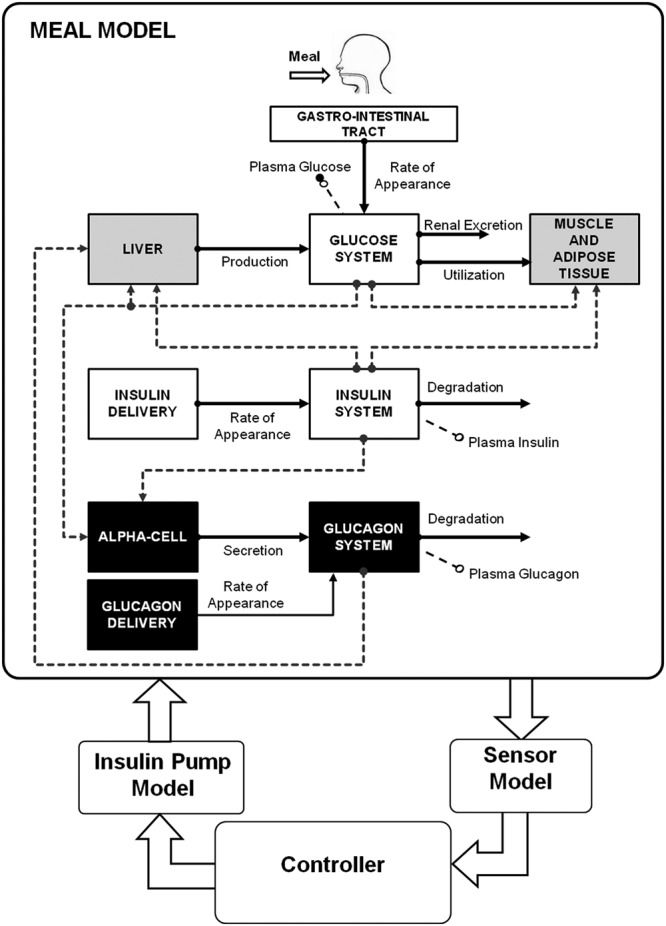
\includegraphics[width=\linewidth]{uvapadova.jpg}
    \caption{UVA/PADOVA equations, visualised}
    \label{fig:uvapadova}
\end{figure}

UVA/Padova \cite{sim-diabetes-fda} is a set of equations used to model type 1 diabetes.
The equations, outlined on figure \ref{fig:uvapadova}, were developed by clinical experts and validated on a dataset of 32 people aged 38 ± 12 years.
It is widely used in Healthcare and even approved in the United States as a replacement for clinical trials.
It provides $p_o(o | s, a)$ and $p_s(s_\text{next} | s_\text{prev}, a)$ (see section \ref{sec:scope}), so to be a full-fledged Markov Decision Process it only need $p_r(r|s,a)$.
\cite{simglucose} solves exactly that by adding a reward function based on diabetes risk index as defined in \cite{diabetesrisk} to the UVA/Padova simulator, providing a Reinforcement Learning environment for type 1 diabetes.

\subsection{GYMIC}
\label{sec:gymic}

\subsubsection{Scope}
GYMIC \cite{gymic} is, unlike the previous examples, a fully data-driven simulator. 
It harnesses a subset of MIMIC \cite{mimic} dataset to address on one of the most challenging problems in emergency care - sepsis.
The authors intentionally limit their scope to just sepsis in order to simplify the modelling task as well as because sepsis prevention has been identified as an area where doctors would particularly benefit from electronic decision support \cite{sepsis-motivation1,sepsis-motivation2}.

\subsubsection{Prediction model}
The prediction model of GYMIC simulator is defined as a solution to the following autoregression task:
\begin{enumerate}
    \item A clinical history is a sequence of $(s, a)$ tuples
    \item $a \in 0,\dots 24$ is one of 25 possible vasopressor or intravenous fluid interventions - a cartensian product of 5 types of interventions and 5 dosage quantiles. 
    \item $s \in R^{46}$ is the patient's state at the moment this intervention was administered.
    \item Predict the conditional state distribution $p_s(s_t, a_t | s_{t-1},s_{t-2},\dots,s_1)$
\end{enumerate}

The dataset of clinical histories is produced by a preprocessing algorithm combining together all clinical records from MIMIC that relate to sepsis patients.

Autoregressive tasks of this nature arise in many fields like stock market prediction \cite{stonks1,stonks2} or language modelling \cite{langmodels} where state of the art solutions can be found.
The authors of \emph{GYMIC} solve it with an LSTM \cite{hochreiterLongShorttermMemory1997} neural network with 2 additional dense layers attached, see figure \ref{fig:gymic} for the diagram.
Faced with some of the mode collapse issues described in section \ref{sec:gymic-results} the authors also experimented with semi-supervised learning \cite{semi-supervised}: they trained a variational autoencoder \cite{vae} on all patient states to replace the 46-vector representations of patient state $s$ with learned representations from the latent space of the VAE $\text{encoder}(s)$.
The issues persisted.

\begin{figure}
    \centering
    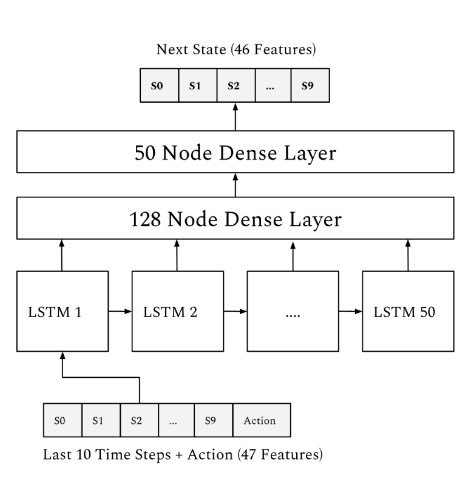
\includegraphics[width=\linewidth]{gymic.png}
    \caption{Neural architecture of GYMIC}
    \label{fig:gymic}
\end{figure}

\subsubsection{Reward model}

Highlighting the gravity of contracting sepsis, \emph{GYMIC} has only 2 outcomes: patient is discharged from intensive care or patient dies.
Its reward model reflects that, giving the agent a large positive or negative reward at the end of the episode, depending on the outcome.
However, in order to lower the difficulty of the simulator (delayed gratification makes training significantly harder \cite{delayedgrat-humans,gulwaniProgramSynthesis2017}) an additional reward is provided during the episode, based on the evolution of the patient's SOFA score \cite{sofa} - a commonly used measure of sepsis severity:

\begin{multline}
r\left(s_{t}, s_{t+1}\right)=C_{0} \mathbb{1}\left(s_{t+1}^{\mathrm{SOFA}}=s_{t}^{\mathrm{SOFA}} \& s_{t+1}^{\text{SOFA }}>0\right) + \\ +
C_{1}\left(s_{t+1}^{\mathrm{SOFA}}-s_{t}^{\mathrm{SOFA}}\right) + 
C_{2} \tanh \left(s_{t+1}^{\text{Lactate }}-s_{t}^{\text{Lactate }}\right)
\end{multline}

A third reward component is proposed to negatively reinforce action severity and encourage the agent to use low doses of drugs - an instance of \emph{confirmation bias} as discussed in section \ref{sec:bias}, but a necessary step given the issues in section \ref{sec:gymic-results}.

\subsubsection{Results and issues}
\label{sec:gymic-results}

Unfortunately, the experiments performed by the authors of \emph{GYMIC} indicate extreme overfitting.
Due to \emph{sampling bias} and simply inadequate size of the dataset there are treatments that have only occurred a few times in the training data and have always resulted in a positive health outcome.
In \emph{GYMIC} these treatments are silver bullets that guarantee a successful outcome while in real life they are risky and potentially very harmful.
